% LaTeX source for textbook ``Physical Modeling in Octave''
% Copyright 2011 Allen B. Downey, Geoff Pleiss

% Permission is granted to copy, distribute and/or modify this
% document under the terms of the GNU Free Documentation License,
% Version 1.1 or any later version published by the Free Software
% Foundation; with the Invariant Sections being "Contributor List",
% with no Front-Cover Texts, and with no Back-Cover Texts. A copy of
% the license is included in the section entitled "GNU Free
% Documentation License".

% You can obtain a copy of the GNU Free Documentation License
% from www.gnu.org or by writing to the Free Software Foundation,
% Inc., 59 Temple Place - Suite 330, Boston, MA 02111-1307, USA.
%
\documentclass{book}
\usepackage{fancyhdr}
\usepackage{graphicx}
\usepackage{url}
\usepackage{makeidx}
\usepackage[symbol*]{footmisc}
\usepackage{amsmath, amsthm, amssymb}
\usepackage{hevea}              
\usepackage{upquote}
%\usepackage{epstopdf}
\usepackage{hyperref} % Maybe? it makes things cool


% Book information
\newcommand{\thetitle}{Physical Modeling in Octave\myreg}
\newcommand{\theauthor}{Geoffrey Pleiss}
\newcommand{\theversion}{1.1.4}


\sloppy
\pagestyle{fancyplain}

\newcommand{\myreg}{\textsuperscript{{\tiny \textregistered}}}
\renewcommand{\chaptermark}[1]{\markboth{#1}{}}
\renewcommand{\sectionmark}[1]{\markright{\thesection\ #1}{}}
\renewcommand\MakeUppercase{}

\lhead[\fancyplain{}{\bfseries\thepage}]%
   {\fancyplain{}{\bfseries\rightmark}}
\rhead[\fancyplain{}{\bfseries\leftmark}]%
   {\fancyplain{}{\bfseries\thepage}}
\cfoot{}

\newenvironment{code}{\vspace{0.6\parskip} \begin{verbatim}}{\end{verbatim} \vspace{0.6\parskip}}

% TODO: get the styles to work
% these styles get translated in CSS for the HTML version
\newstyle{a:link}{color:black;}
\newstyle{p+p}{margin-top:1em;margin-bottom:1em}
\newstyle{img}{border:0px}

% change the arrows
%\setlinkstext
% {\imgsrc[ALT="Previous"]{html/back.png}}
% {\imgsrc[ALT="Up"]{html/up.png}}
% {\imgsrc[ALT="Next"]{html/next.png}}

%% Theorem styles
\newtheoremstyle{myex}% name
   {9pt}%   Space above
   {9pt}%   Space below
   {\itshape}%     Body font
   {}%     Indent amount (empty = no indent, \parindent = para indent)
   {\bfseries}% Thm head font
   {}%    Punctuation after thm head
   {9pt}%   Space after thm head: " " = normal interword space;
      %    \newline = linebreak
   {}%     Thm head spec (can be left empty, meaning `normal')

\theoremstyle{myex}
\newtheorem{ex}{Exercise}[chapter]
\makeindex


\begin{document}

\title {\thetitle}
\author {\theauthor}
\date {Version \theversion}


% % Title and copyright page - for both latex and html
\input{latexonly}
% \input{htmlonly}
\begin{latexonly}

%\blankpage
%\blankpage

% TITLE PAGES FOR LATEX VERSION

\maketitle

\vspace{2in}

\begin{center}
{\Large \thetitle}

\vspace{0.25in}

Copyright 2007, 2008, 2009, 2010 Allen B. Downey
\end{center}

\vspace{0.25in}

Permission is granted to copy, distribute and/or modify this
document under the terms of the GNU Free Documentation License,
Version 1.1 or any later version published by the Free Software
Foundation; this book contains no Invariant Sections,
no Front-Cover Texts, and no Back-Cover Texts.

You can obtain a copy of the GNU Free Documentation License
from www.gnu.org or by writing to the Free Software Foundation,
Inc., 59 Temple Place - Suite 330, Boston, MA 02111-1307, USA.

The original form of this book is LaTeX source code.
Compiling this LaTeX source has the effect of generating
a device-independent representation of a book, which
can be converted to other formats and printed.

This book was typeset by the author using latex, dvips and ps2pdf,
among other free, open-source programs.
The LaTeX source for this book is available from
\url{http://greenteapress.com/matlab}.

Octave\myreg is a registered trademark of The
Mathworks, Inc. The Mathworks does not warrant the accuracy
of this book; they probably don't even like it.

\frontmatter

\end{latexonly}





% HTMLONLY

\begin{htmlonly}

% TITLE PAGE FOR HTML VERSION

{\Large \thetitle}

{\large Allen B. Downey}

Version \theversion

\setcounter{chapter}{-1}

Copyright 2010 Allen B. Downey

\vspace{0.25in}

Permission is granted to copy, distribute and/or modify this document
under the terms of the Creative Commons Attribution-Share Alike 3.0
Unported License, which is available at
\url{creativecommons.org/licenses/by-sa/3.0/}.

\end{htmlonly}


% % Preface
% Preface

\chapter*{Preface}

Most books that use Octave are aimed at readers who know how
to program. This book is for people who have never programmed
before.

As a result, the order of presentation is unusual. The book starts
with scalar values and works up to vectors and matrices very
gradually. This approach is good for beginning programmers, because
it is hard to understand composite objects until you understand basic
programming semantics. But there are problems:

\begin{itemize}

\item The Octave documentation is written in terms of matrices,
and so are the error messages.
To mitigate this problem, the book explains the necessary
vocabulary early and deciphers some of the messages that
beginners find confusing.

\item Many of the examples in the first half of the book are
not idiomatic Octave. I address this problem in the second
half by translating the examples into a more standard style.

\end{itemize}

The book puts a lot of emphasis on functions, in part because they are
an important mechanism for controlling program complexity, and also
because they are useful for working with Octave tools like {\tt fzero}
and {\tt ode45}.

I assume that readers know calculus, differential equations, and
physics, but not linear algebra. I explain the math as I go along,
but the descriptions might not be enough for someone who hasn't seen
the material before.

There are small exercises within each chapter, and a few larger
exercises at the end of some chapters.

This is Version 1.1 of the book. I used Version 0.9 for my class
in Fall 2007. I made some corrections based on feedback from students
and others, then added some exercises and additional chapters.
If you have suggestions and corrections, please send them to
{\tt downey@allendowney.com}.

\noindent Allen B. Downey \\
\noindent Needham, MA \\
\noindent December 28, 2007

\vspace{0.1in}

\section*{Contributor's list}

The following are some of the people who have contributed to this
book:

\begin{itemize}

\item Michael Lintz spotted the first (of many) typos.

\item Kaelyn Stadtmueller reminded me of the importance of linking
verbs.

\item Roydan Ongie knows a matrix when he sees one (and caught a typo).

\item Keerthik Omanakuttan knows that acceleration is not the
second derivative of acceleration.

\item Pietro Peterlongo pointed out that Binet's formula is an
exact expression for the $n$th Fibonacci number, not an approximation.

\item Li Tao pointed out several errors.

\item Steven Zhang pointed out an error and a point of confusion
in Chapter 11.

\item Elena Oleynikova pointed out the ``gotcha'' that script file names
can't have spaces.

\item Kelsey Breseman pointed out that numbers as footnote markers
can be confused with exponents, so now I am using symbols.

\item Philip Loh sent me some updates for recent revisions of Octave.

\item Harold Jaffe spotted a typo.

\item Vidie Pong pointed out the problem with spaces in filenames.

\end{itemize}

% ENDCONTRIB


% % Table of contents
\tableofcontents


%%%%%%%%%%%%%%%%%%%%%%%%%%
%STARTED WORK HERE 1-31-11
%%%%%%%%%%%%%%%%%%%%%%%%%%
\mainmatter


% % chap01 - Variables and values
% chap01 - Variables and values
% Last edited: 08-24-11 by Geoff

\chapter{Variables and values}

\section{A glorified calculator}
\label{calc}

At heart, Octave is a glorified calculator. Technically, Octave is a
program for {\bf scientific computing} -- constructing mathematical models
to solve scientific problems.
% Is this a good definition?
What this boils down to is a calculator with extended capabilities.

The Octave application is nothing more than an {\bf interpereter}. You supply
the program with an Octave {\bf command}, such as an expression or function,
and the program will execute the command and print the result. This is no
different than you typing {\tt 2 + 3} into a calculator and having it print
out {\tt 5}.

Starting up the Octave application will open up a terminal window.
(In certain operating systems, you can start up Octave by typing the command
{\tt octave} in an existing terminal window). This terminal window is now the
Octave command window, and the last line should look something
like this:
%
\begin{verbatim}
octave:1>
\end{verbatim}
%
This is the Octave {\bf prompt}; that is, the line that prompts you to
enter a command. (The number after the colon represents the current
command
number. After you execute your first command, the prompt will read {\tt
octave:2>}, etc.). Your prompt may look different than this, depending on what
operating system you're using.

The simplest kind of command is a mathematical {\bf expression}, which
is made up of {\bf operands} (like numbers, for example) and
{\bf operators} (like the plus sign, {\tt +}).

If you type an expression and then press Enter (or Return), Octave
{\bf evaluates} the expression and prints the result.

\begin{verbatim}
octave:1> 2 + 1
ans = 3
octave:2>
\end{verbatim}

Just to be clear: in the example above, Octave printed {\tt octave:1>} ; I
typed {\tt 2 + 1} and then hit Enter, and Octave printed {\tt ans = 3}.
And when I say ``printed,'' I really mean ``displayed on the screen,''
which might be confusing, but it's the way people talk. Octave also printed
{\tt octave:2>}, which is the prompt for your next command.

An expression can contain any number of operators and operands. You
don't have to put spaces between them; some people do and some people
don't.

\begin{verbatim}
octave:2> 1+2+3+4+5+6+7+8+9
ans = 45
\end{verbatim}

The other arithmetic operators are pretty much what you would expect.
Subtraction is denoted by a minus sign, {\tt -}; multiplication by
an asterisk, {\tt *} (sometimes pronounced ``splat''); division by
a forward slash, {\tt /}.

\begin{verbatim}
octave:3> 2*3 - 4/5
ans = 5.2000
\end{verbatim}

The order of operations is what you would expect from basic algebra:
multiplication and division happen before addition and subtraction.
If you want to override the order of operations, you can use parentheses.

\begin{verbatim}
octave:4> 2 * (3-4) / 5
ans = -0.4000
\end{verbatim}

When I added the parentheses I also changed the spacing to make the
grouping of operands clearer to a human reader. This is the first
of many style guidelines I will recommend for making your programs
easier to read. Style doesn't change what the program does; the Octave
interpreter doesn't check for style. But human readers do, and the
most important human who will read your code is you.

And that brings us to the First Theorem of debugging:

\begin{quote}
Readable code is debuggable code.
\end{quote}

It is worth spending time to make your code pretty; it will save
you time debugging!

The other common operator is exponentiation, which uses the \verb+^+
symbol, sometimes pronounced ``carat'' or ``hat''. So 2 raised to the
16th power is

\begin{verbatim}
octave:5> 2^16
ans = 65536
\end{verbatim}

As in basic algebra, exponentiation happens before multiplication
and division, but again, you can use parentheses to override the order
of operations.

You now know enough commands to use Octave as a basic calculator! To quit the
application, either close the terminal window, or type the command {\tt quit}
at the prompt. (The command {\tt exit} will also work).


\section{Math functions}

Octave's functionality goes well beyond simple math operations -- it knows how
to compute pretty much every math function you've
heard of. Octave knows all the trigonometric functions; here's how you
use them:

\begin{verbatim}
octave:1> sin(1)
ans = 0.8415
\end{verbatim}

This command is an example of a {\bf function call}. The name of the
function is {\tt sin}, which is the usual abbreviation for the
trigonometric sine. The value in parentheses is called the {\bf argument}.
All the trig functions in Octave work in radians.

All functions in Octave are case-sensitive. In other words, typing {\tt Sin(1)}
will give you an error.

\begin{verbatim}
octave:2> Sin(1)
error: `Sin' undefined near line 2 column 1
\end{verbatim}

Some functions take more than one argument, in which case they are
separated by commas. For example, {\tt atan2} computes the inverse
tangent, which is the angle in radians between the positive x-axis and
the point with the given $y$ and $x$ coordinates.

\begin{verbatim}
octave:3> atan2(1,1)
ans = 0.7854
\end{verbatim}

If that bit of trigonometry isn't familiar to you, don't worry about
it. It's just an example of a function with multiple arguments.

Octave also provides exponential functions, like {\tt exp}, which
computes $e$ raised to the given power. So {\tt exp(1)} is just $e$.

\begin{verbatim}
octave:4> exp(1)
ans = 2.7183
\end{verbatim}

The inverse of {\tt exp} is {\tt log}, which computes the logarithm
base $e$:

\begin{verbatim}
octave:5> log(exp(3))
ans = 3
\end{verbatim}

This example also demonstrates that function calls can be {\bf nested};
that is, you can use the result from one function as an argument for
another.

More generally, you can use a function call as an operand in an expression.

\begin{verbatim}
octave:5> sqrt(sin(0.5)^2 + cos(0.5)^2)
ans = 1
\end{verbatim}

As you probably guessed, {\tt sqrt} computes the square root.

There are lots of other math functions, but this is not meant to
be a reference manual. To learn about other functions, you should
read the documentation.


\section{Documentation}

Octave has exenstive written documents, both online and printed resources,
that outline every feature and command. However, often you just want to know
how to use one command or function. Fortunatly, the Octave program has a
built-in help command:
{\tt help}.

The help command works from the Command Window; just type {\tt help}
followed by the name of a command.

\begin{verbatim}
octave:1> help sin
`sin' is a built-in function

 -- Mapping Function:  sin (X)
     Compute the sine for each element of X in radians.

     See also: asin, sind, sinh
\end{verbatim}

In general, help pages are fairly simple to use, although they will use some
vocabulary you don't know yet. For example, ``for each element of X'' won't make
sense until we get to vectors and matricies a few chapters from now.

Another downside of the help pages is that there are no examples. Some of the
functions may be simple enough to use without examples, but for others it
may be difficult. You can find some examples found in the online Octave guide,
which can be found at \url{http://www.gnu.org/software/octave/docs.html}.
Unfortunatly, this guide can be a little difficult to navigate, especially when
you're getting started.

The help command only works when you know the exact name of the command you are
looking up. What happens if you don't know the exact name? For example, let's
say you want to find the eigenvalues of a matrix. You know that Octave has a
function for calculating eigenvalues, but you don't know it's name. If you enter
the command {\tt help eigenvalues}, you will get an error message.

\begin{verbatim}
octave:2> help eigenvalues
error: help: `eigenvalues' not found
\end{verbatim}

How do you find out the name of the eigenvalues function? This is where
{\tt lookfor} comes into play. The lookfor command will search through
all of the help pages and give you a list of commands with that search term. So
if you were to type {\tt lookfor eigenvalues}, you'd get:

\begin{verbatim}
octave:2> lookfor eigenvalues
eig                 The eigenvalues (and eigenvectors) of a matrix 
                    are computed in a several step pr
eigs                Calculate a limited number of eigenvalues and
                    eigenvectors of A, based on a sele
schur               The Schur decomposition is used to compute 
                    eigenvalues of a square matrix, and h
\end{verbatim}

Remember, the lookfor command has a lot of help pages to look through, so it
may take a while for it to print out results. Also, the search
terms are NOT case-sensitive, so {\tt lookfor eigenvalues} will produce the
same search results as {\tt lookfor Eigenvalues}.

What happens if Octave can't display all of a help page at once? Try entering
the command {\tt help plot}. Chances are (unless you have a really really big
monitor), your terminal should display something like this:
%Is this the best way to do this?

\begin{verbatim}
`plot' is a function from the file /usr/share/octave/3.2.3/m/plot/plot.m

 -- Function File:  plot (Y)
 -- Function File:  plot (X, Y)
 -- Function File:  plot (X, Y, PROPERTY, VALUE, ...)
 -- Function File:  plot (X, Y, FMT)
 -- Function File:  plot (H, ...)
     Produces two-dimensional plots.  Many different combinations of
     arguments are possible.  The simplest form is

          plot (Y)

     where the argument is taken as the set of Y coordinates and the X
     coordinates are taken to be the indices of the elements, starting
     with 1.

     To save a plot, in one of several image formats such as PostScript
     or PNG, use the `print' command.

     If more than one argument is given, they are interpreted as

          plot (Y, PROPERTY, VALUE, ...)

:
\end{verbatim}

Notice that you can no longer access your prompt. Don't worry, it's still there.
What's happened is Octave has opened up a {\it pager}, which is a process used
for viewing large amounts of text. Press the ENTER key to go forward on
line, or press SPACE to go forward a window's worth of text. To go
backwards, press B. Press P to go back up to the top of the page.
To exit the pager and return to the prompt, press Q. When you exit the pager,
all of the text from the help page disappears, and you are back where you left
off.

\begin{verbatim}
octave:3> help plot
octave:4>
\end{verbatim}

Octave uses pagers whenever the output from a command is too big to fit in one
window, so don't be surprised if you see one when you enter a command like {\tt
1:1000}. (We'll learn what that command means in chapter 3.)

There are more ways to access to access Octave's help files and documentation.
You can read about them on the online guide.


\section{Variables}

One of the features that makes Octave more powerful than a calculator
is the ability to give a name to a value. A named value is called
a {\bf variable}.

Octave comes with a few predefined variables. For
example\footnote{Technically {\tt pi} is a function, not a variable,
but for now it's best to pretend.}, the name {\tt pi} refers to the
mathematical quantity $\pi$, which is approximately

\begin{verbatim}
octave:1> pi
ans = 3.1416
\end{verbatim}

And if you do anything with complex numbers, you might find it
convenient that both {\tt i} and {\tt j} are predefined as the square
root of $-1$.

You can use a variable name anywhere you can use a number; for example, as
an operand in an expression:

\begin{verbatim}
octave:2> pi * 3^2
ans = 28.274
\end{verbatim}

or as an argument to a function:

\begin{verbatim}
octave:3> sin(pi/2)
ans = 1
octave:4> exp(i * pi)
ans = -1.0000e+00 + 1.2246e-16i
\end{verbatim}

As the second example shows, many Octave functions work with
complex numbers. This example demonstrates Euler's Equality:
$e^{i \pi} = -1$.\footnote{Actually, this answer has a small imaginary
component, but this is due to the method that Octave uses to calculate the
exponential function. $1.2246 \times 10^{-16}$ is very very small, so for all
intents and purposes we can assume that it is zero.}

Whenever you evaluate an expression, Octave assigns the result to
a variable named {\tt ans}. You can use {\tt ans} in a subsequent
calculation as shorthand for ``the value of the previous expression.''

\begin{verbatim}
octave:5> 3^2 + 4^2
ans = 25
octave:6> sqrt(ans)
ans = 5
\end{verbatim}

But keep in mind that the value of {\tt ans} changes every time
you evaluate an expression.


\section{Assignment statements}

You can create your own variables, and give them values, with
an {\bf assignment statement}. The assignment operator is the
equals sign, {\tt =}.

\begin{verbatim}
octave:1> x = 6 * 7
x = 42
\end{verbatim}

This example creates a new variable named {\tt x} and assigns it the
value of the expression {\tt 6 * 7}. Octave responds with the
variable name and the computed value.

In every assignment statement, the left side has to be a
legal variable name. The right side can be any expression,
including function calls.

Almost any sequence of lower and upper case letters is a legal
variable name. Some punctuation is also legal, but the underscore,
{\tt \_}, is the only commonly-used non-letter. Numbers are fine, but
not at the beginning. Spaces are not allowed. Variable names are
``case sensitive'', so {\tt x} and {\tt X} are different variables.

\begin{verbatim}
octave:2> fibonacci0 = 1;
octave:3> LENGTH = 10;
octave:4> first_name = 'allen'
first_name = allen
\end{verbatim}

The first two examples demonstrate the use of the semi-colon, which
suppresses the output from a command. In this case Octave creates the
variables and assigns them values, but displays nothing.

The third example demonstrates that not everything
in Octave is a number. A sequence of characters in single quotes is
a {\bf string}.

Although {\tt i}, {\tt j} and {\tt pi} are predefined, you are free
to reassign them. It is common to use {\tt i} and {\tt j} for other
purposes, but it is probably not a good idea to change the value of
{\tt pi}!

\section{Why variables?}

The most common reasons to use variables are

\begin{itemize}

\item To avoid recomputing a value that is used repeatedly. For
example, if you are performing computations involving $e$, you might
want to compute it once and save the result.

\begin{verbatim}
octave:1> e = exp(1)
e = 2.7183
\end{verbatim}


\item To make the connection between the code and the underlying
mathematics more apparent. If you are computing the area of a circle,
you might want to use a variable named {\tt r}:

\begin{verbatim}
octave:2> r = 3
r = 3
octave:3> area = pi * r^2
area = 28.2743
\end{verbatim}

That way your code resembles the familiar formula $\pi r^2$.

\item To break a long computation into a sequence of steps.
Suppose you are evaluating a big, hairy expression like this:

\begin{verbatim}
octave:4> ans = ((x - theta) * sqrt(2 * pi) * sigma) ^ -1 * ...
> exp(-1/2 * (log(x - theta) - zeta)^2 / sigma^2)
\end{verbatim}

You can use an ellipsis to break the expression into multiple lines.
Just type {\tt ...} at the end of the first line and
continue on the next. (Octave prints the {\tt >} on the next line).

But often it is better to break the computation into a sequence of
steps and assign intermediate results to variables.

\begin{verbatim}
shiftx = x - theta
denom = shiftx * sqrt(2 * pi) * sigma
temp = (log(shiftx) - zeta) / sigma
exponent = -1/2 * temp^2
ans = exp(exponent) / denom
\end{verbatim}

The names of the intermediate variables explain their role in the
computation. {\tt shiftx} is the value of {\tt x} shifted by {\tt
theta}. It should be no surprise that {\tt exponent} is the argument
of {\tt exp}, and {\tt denom} ends up in the denominator. Choosing
informative names makes the code easier to read and understand (see
the First Theorem of Debugging).

\end{itemize}


\section{Errors}

It's early, but now would be a good time to start making errors.
Whenever you learn a new feature, you should try
to make as many errors as possible, as soon as possible.

When you make deliberate errors, you get to see what the error messages
look like. Later, when you make accidental errors, you will know what
the messages mean.

A common error for beginning programmers is leaving out the {\tt *}
for multiplication.

\begin{verbatim}
octave:1> area = pi r^2
parse error:

  syntax error

>>> area = pi r^2
              ^
\end{verbatim}

The error message indicates that, after seeing the operand {\tt pi},
Octave was ``expecting'' to see an operator, like {\tt *}. Instead,
it got a variable name, which is the ``syntax error'' indicated
by the carat (\verb+^+).

Another common error is to leave out the parentheses around the
arguments of a function. For example, in math notation, it is common
to write something like $\sin \pi$, but not in Octave.

\begin{verbatim}
octave:1> sin pi
error: octave_base_value::sin (): wrong type argument `sq_string'
\end{verbatim}

The problem is that when you leave out the parentheses, Octave treats
the argument as a string (rather than as an expression). In
this case the {\tt sin} function generates a reasonable error message,
but in other cases the results can be baffling. For example, what
do you think is going on here?

\begin{verbatim}
octave:1> abs pi
ans =
   112   105
\end{verbatim}

There is a reason for this ``feature'', but rather than get into that
now, let me suggest that you should {\em always} put parentheses around
arguments.

This example also demonstrates the Second Theorem of Debugging:

\begin{quote}
The only thing worse than getting an error message is {\em not}
getting an error message.
\end{quote}

Beginning programmers hate error messages and do everything they
can to make them go away. Experienced programmers know that error
messages are your friend. They can be hard to understand, and even
misleading, but it is worth making some effort to understand them.

Here's another common rookie error. If you were translating
the following mathematical
expression into Octave:

\[ \frac{1}{2 \sqrt \pi}\]

You might be tempted to write something like this:

\begin{verbatim}
1 / 2 * sqrt(pi)
\end{verbatim}

But that would be wrong. So very wrong.


\section{Floating-point arithmetic}

In mathematics, there are several kinds of numbers: integer, real,
rational, irrational, imaginary, complex, etc. Octave only has one
kind of number, called {\bf floating-point}.

You might have noticed that Octave expresses values in decimal
notation. So, for example, the rational number $1/3$ is represented
by the floating-point value

\begin{verbatim}
octave:1> 1/3
ans = 0.3333
\end{verbatim}

which is only approximately correct. It's not quite as bad as
it seems; Octave uses more digits than it shows by default.
You can change the {\tt format} to see the other digits.

\begin{verbatim}
octave:2> format long
octave:3> 1/3
ans =  0.333333333333333
\end{verbatim}

Internally, Octave uses the IEEE double-precision floating-point
format, which provides about 15 significant digits of precision (in
base 10). Leading and trailing zeros don't count as ``significant''
digits, so Octave can represent large and small numbers
with the same precision.

Very large and very small values are displayed in scientific notation.

\begin{verbatim}
octave:4> factorial(100)
ans =  9.33262154439422e+157
\end{verbatim}

The {\tt e} in this notation is {\em not} the transcendental number
known as $e$; it is just an abbreviation for ``exponent''. So
this means that $100!$ is approximately $9.33 \times 10^{157}$. The
exact solution is a 158-digit integer, but we only know the first 16
digits.

You can enter numbers using the same notation.

\begin{verbatim}
octave:5> speed_of_light = 3.0e8
speed_of_light = 300000000
\end{verbatim}

Although Octave can handle large numbers, there is a limit. The
predefined variables {\tt realmax} and {\tt realmin} contain the
largest and smallest numbers that Octave can handle\footnote{The names
of these variables are misleading; floating-point numbers are
sometimes, wrongly, called ``real''.}.

\begin{verbatim}
octave:6> realmax
ans =  1.79769313486232e+308
octave:7> realmin
ans =  2.22507385850720e-308
\end{verbatim}

If the result of a computation is too big, Octave ``rounds up''
to infinity.

\begin{verbatim}
octave:8> factorial(170)
ans =  7.25741561530806e+306
octave:9> factorial(171)
ans = Inf
\end{verbatim}

Division by zero also returns {\tt Inf}, but in this case Octave
gives you a warning because division by zero is usually
considered undefined.

\begin{verbatim}
octave:10> 1/0
warning: division by zero
ans = Inf
\end{verbatim}

A warning is like an error message without teeth; the computation
is allowed to continue. Allowing {\tt Inf} to propagate
through a computation doesn't always do what you expect, but if you
are caul with how you use it, {\tt Inf} can be quite useful.

For operations that are truly undefined, Octave returns {\tt NaN},
which stands for ``not a number''.

\begin{verbatim}
octave:11> 0/0
warning: division by zero
ans = NaN
\end{verbatim}


\section{Comments}

Along with the commands that make up a program, it is useful
to include comments that provide additional information about the
program. The percent symbol {\tt \%} separates
the comments from the code.

\begin{verbatim}
octave:1> speed_of_light = 3.0e8   % meters per second
speed_of_light = 300000000
\end{verbatim}

The comment runs from the percent symbol to the end of the line.
In this case it specifies the units of the value. In an ideal world,
Octave would keep track of units and propagate them through the
computation, but for now that burden falls on the programmer.

Comments have no effect on the execution of the program. They
are there for human readers. Good comments make programs more
readable, but bad comments are useless or (even worse) misleading.

Avoid comments that are redundant with the code:

\begin{verbatim}
octave:2> x = 5    % assign the value 5 to x
\end{verbatim}

Good comments provide additional information that is not in the
code, like units in the example above, or the meaning of a variable:

\begin{verbatim}
octave:3> p = 0;   % position from the origin in meters 
octvae:4> v = 100;   % velocity in meters / second
octave:5> a = -9.8;  % acceleration of gravity in meters / second^2
\end{verbatim}

If you use longer variable names, you might not need explanatory
comments, but there is a tradeoff: longer code can become harder
to read. Also, if you are translating from math
that uses short variable names, it can be useful to make your
program consistent with your math. 

\section{Glossary}

\begin{description}

\item[scientific computing:] A field of study based around constructing
mathematical models to solve physical problems.

\item[interpreter:] The program that reads and executes Octave code.

\item[command:] A line of Octave code executed by the interpreter.

\item[prompt:] The symbol the interpreter prints to indicate that it is
waiting for you to type a command.

\item[operator:] One of the symbols, like {\tt *} and {\tt +}, that
represent mathematical operations.  

\item[operand:] A number or variable that appears in an expression along
with operators.

\item[expression:] A sequence of operands and operators that specifies
a mathematical computation and yields a value.  

\item[value:] The numerical result of a computation.  

\item[evaluate:] To compute the value of an expression.  

\item[order of operations:] The rules that specify which operations
in an expression are performed first.

\item[function:] A named computation; for example {\tt log10} is the
name of a function that computes logarithms in base 10.

\item[call:] To cause a function to execute and compute a result.  

\item[function call:] A kind of command that executes a function.  

\item[argument:] An expression that appears in a function call to
specify the value the function operates on.

\item[nested function call:] An expression that uses the result from
one function call as an argument for another.  

\item[variable:] A named value.  

\item[assignment statement:] A command that creates a new variable
(if necessary) and gives it a value.

\item[string:] A value that consists of a sequence of characters (as
opposed to a number). 

\item[floating-point:] The kind of number Octave works with. All
floating-point numbers can be represented with about 16 significant
decimal digits (unlike mathematical integers and reals).

\item[scientific notation:] A format for typing and displaying large
and small numbers; e.g. {\tt 3.0e8}, which represents $3.0 \times 10^8$
or 300,000,000. 

\item[comment:] Part of a program that provides additional information
about the program, but does not affect its execution. 

\end{description}


\section{Exercises}

\begin{ex}
Write a Octave expression that evaluates the
following math expression. You can assume that the variables
{\tt mu}, {\tt sigma} and {\tt x} already exist.

\begin{equation}
\frac{e^{- \left( \frac{x-\mu}{\sigma \sqrt{}2} \right) ^2}}
{\sigma \sqrt{2 \pi}}
\end{equation}

Note: you can't use Greek letters in Octave; when translating
math expressions with Greek letters, it is common to write out
the name of the letter (assuming you know it).
\end{ex}


% 
% % chap02 - Scripts
\include{chapters/scripts}
% 
% % chap03 - Loops
% chap03 - Loops
% Last edited:

\chapter{Loops}

\section{Updating variables}

In Exercise~\ref{cargame}, you might have been tempted to write something
like

\begin{verbatim}
a = a - 0.05*a + 0.03*b
b = b + 0.05*a - 0.03*b
\end{verbatim}

But that would be wrong, so very wrong. Why? The problem is that
the first line changes the value of {\tt a}, so when the second line
runs, it gets the old value of {\tt b} and the new value of {\tt a}.
As a result, the change in {\tt a} is not always the same as the
change in {\tt b}, which violates the principle of Conversation
of Cars!

One solution is to use temporary variables {\tt anew} and {\tt bnew}:

\begin{verbatim}
anew = a - 0.05*a + 0.03*b
bnew = b + 0.05*a - 0.03*b
a = anew
b = bnew
\end{verbatim}

This has the effect of updating the variables ``simultaneously;'' that
is, it reads both old values before writing either new value.

The following is an alternative solution that
has the added advantage of simplifying the computation:

\begin{verbatim}
atob = 0.05*a - 0.03*b
a = a - atob
b = b + atob
\end{verbatim}

It is easy to look at this code and confirm that it obeys Conversation
of Cars. Even if the value of {\tt atob} is wrong, at least the total
number of cars is right. And that brings us to the Seventh Theorem of
Debugging:

\begin{quote}
The best way to avoid a bug is to make it impossible.
\end{quote}

In this case, removing redundancy also eliminates the opportunity for
a bug.


\section{Kinds of error}

There are four kinds of error:

\begin{description}

\item[Syntax error:] You have written a Octave command that cannot
execute because it violates one of the rules of syntax. For example,
you can't have two operands in a row without an operator, so 
\verb+pi r^2+ contains a syntax error. When Octave finds a syntax
error, it prints an error message and stops running your program.

\item[Runtime error:] Your program starts running, but something goes
wrong along the way. For example, if you try to access a variable
that doesn't exist, that's a runtime error. When Octave detects the
problem, it prints an error message and stops.

\item[Logical error:] Your program runs without generating any error
messages, but it doesn't do the right thing. The problem in the
previous section, where we changed the value of {\tt a} before
reading the old value, is a logical error.

\item[Numerical error:] Most computations in Octave are only
approximately right. Most of the time the errors are small enough
that we don't care, but in some cases the roundoff errors are a problem.

\end{description}

Syntax errors are usually the easiest. Sometimes the error messages
are confusing, but Octave can usually tell you where the error is, at
least roughly.

Run time errors are harder because, as I mentioned before, Octave
can tell you where it detected the problem, but not what caused it.

Logical errors are hard because Octave can't help at all. Only you
know what the program is supposed to do, so only you can check it.
From Octave's point of view, there's nothing wrong with the program;
the bug is in your head!

Numerical errors can be tricky because it's not clear whether the
problem is your fault. For most simple computations, Octave produces
the floating-point value that is closest to the exact solution, which
means that the first 15 significant digits should be correct. But some
computations are ill-conditioned, which means that even if your program
is correct, the roundoff errors accumulate and the number of correct
digits can be smaller. Sometimes Octave can warn you that
this is happening, but not always! Precision (the number of digits
in the answer) does not imply accuracy (the number of digits that
are right).


\section{Absolute and relative error}

There are two ways of thinking about numerical errors, called {\bf
absolute} and {\bf relative}.

An absolute error is just the difference between the correct value and
the approximation. We usually write the magnitude of the error,
ignoring its sign, because it doesn't matter whether the approximation
is too high or too low.

For example, we might want to estimate $9!$ using the formula $\sqrt
{18 \pi} ( 9 / e)^9$. The exact answer is $9 \cdot 8 \cdot 7 \cdot 6
\cdot 5 \cdot 4 \cdot 3 \cdot 2 \cdot 1 = 362,880$. The approximation
is $359,536.87$. The absolute error is 3,343.13.

At first glance, that sounds like a lot---we're off by three
thousand---but it is worth taking into account the size of the
thing we are estimating. For example, \$3000 matters a lot
if we are talking about my annual salary, but not at all if we
are talking about the national debt.

A natural way to handle this problem is to use relative
error, which is the error expressed as a fraction (or percentage)
of the exact value. In this case, we would divide the error
by 362,880, yielding $.00921$, which is just less than 1\%.
For many purposes, being off by 1\% is good enough.


\section{for loops}

A {\bf loop} is a part of a program that executes repeatedly;
a {\bf for loop} is the kind of loop that uses the {\tt for}
statement.

The simplest use of a {\tt for} loop is to execute one or more
lines a fixed number of times. 
For example, in the last chapter
we wrote a script named {\tt car\_update} that simulates one
week in the life of a rental car company. To simulate an entire
year, we have to run it 52 times:

\begin{verbatim}
for i=1:52
  car_update
end
\end{verbatim}

The first line looks like an assignment statement, and it {\em is}
like an assignment statement, except that it runs more than once. The
first time it runs, it creates the variable {\tt i} and assigns it the
value 1. The second time, {\tt i} gets the value 2, and so on, up to
52.

The colon operator, {\tt :}, specifies a {\bf range} of integers. In
the spirit of unit testing, you can create a range at the prompt:

\begin{verbatim}
octave:1> 1:5
ans = 1   2   3   4   5
\end{verbatim}

The variable you use in the for statement is called the {\bf loop
variable}. It is a common convention to use the names {\tt i},
{\tt j} and {\tt k} as loop variables.

The statements inside the loop are called the {\bf body}. By convention,
they are indented to show that they are inside the loop, but the
indentation does not actually affect the execution of the program.
The end of the loop is officially marked by the {\tt end} statement.

To see the loop in action you can run a loop that displays the
loop variable:

\begin{verbatim}
octave:2> for i=1:5
> i
> end
i =  1
i =  2
i =  3
i =  4
i =  5
\end{verbatim}

As this example shows, you {\em can} run a for loop from the
command line, but it's much more common to put it in a script.

\begin{ex}
Create a script named {\tt car\_loop} that uses a {\tt for}
loop to run {\tt car\_update} 52 times. Remember that before you run
{\tt car\_update}, you have to assign values to {\tt a} and {\tt b}.
For this exercise, start with the values {\tt a = 150} and {\tt b =
150}.

If everything goes smoothly, your script will display a long stream
of numbers on the screen. But it is probably too long
to fit, and even if it fit, it would be hard to interpret. 
A graph would be much better!
\end{ex}


\section{plotting}
\label{plotting}

{\tt plot} is a versatile function for plotting points and lines
on a two-dimensional graph. Unfortunately, it is so versatile
that it can be hard to use (and hard to read the documentation!).
We will start simple and work our way up.

To plot a single point, type

\begin{verbatim}
octave:1> plot(1, 2)
\end{verbatim}

A {\sf Figure Window} should appear with a graph. You probably won't be able to
see it, but there is a single very small blue dot
at $x$ position 1 and $y$ position 2. To make the dot more visible,
you can specify a different shape:

\begin{verbatim}
octave:2> plot(1, 2, 'o')
\end{verbatim}

The letter in single quotes is a string that specifies how the
point should be plotted. You can also specify the color:

\begin{verbatim}
octave:3> plot(1, 2, 'ro')
\end{verbatim}

{\tt r} stands for red; the other colors include {\bf g}reen, {\bf
b}lue, {\bf c}yan, {\bf m}agenta, {\bf w}hite and blac{\bf k}.
Other shapes include {\tt +}, 
{\tt *}, 
{\tt x}, and 
\verb+^+ (for a triangle). 
We recommend that you specify the shape, if not not the color. The small dot
that Octave uses as a default is normally very difficult to see, where as the
other shapes are fairly visible.

When you use {\tt plot} this way, it can only plot one point at a
time. If you run {\tt plot} again, it clears the figure before making
the new plot. The {\tt hold} command lets you override that behavior.
{\tt hold on} tells Octave not to clear the figure when it makes a new
plot; {\tt hold off} returns to the default behavior.

Try this:

\begin{verbatim}
octave:4> hold on
octave:5> plot(1, 1, 'o')
octave:6> plot(2, 2, 'o')
\end{verbatim}

You should see a figure with two points. Octave scales
the plot automatically so that the axes run from the lowest value in
the plot to the highest. So in this example the points are plotted in
the corners.

\begin{ex}
Modify {\tt car\_loop} so that each time through the
loop it plots the value of {\tt a} versus the value of {\tt i}.

Once you get that working, modify it so it plots the values of {\tt a}
with red circles and the values of {\tt b} with blue diamonds.

\end{ex}

One more thing: if you use {\tt hold on} to prevent Octave from
clearing the figure, you might want to clear the figure yourself,
from time to time, with the command {\tt clf}.


\section{Sequences}

In mathematics a {\bf sequence} is a set of numbers that corresponds
to the positive integers. The numbers in the sequence are
called {\bf elements}. In math notation, the elements
are denoted with subscripts, so the first element of the series $A$ is
$A_1$, followed by $A_2$, and so on.

{\tt for} loops are a natural way to compute the elements of a sequence.
As an example, in a geometric sequence, each element is a constant
multiple of the previous element. As a more specific example, let's
look at the sequence with $A_1 = 1$ and the ratio $A_{i+1} = A_i/2$,
for all $i$. In other words, each element is half as big as the one
before it.

The following loop computes the first 10 elements of $A$:

\begin{verbatim}
a = 1
for i=2:10
  a = a/2
end
\end{verbatim}

Each time through the loop, we find the next value of {\tt a}
by dividing the previous value by 2. Notice that the loop
range starts at 2 because the initial value of {\tt a} corresponds
to $A_1$, so the first time through the loop we are computing
$A_2$.

Each time through the loop, we replace the previous element with
the next, so at the end, {\tt a} contains the 10th element. The
other elements are displayed on the screen, but they are not saved
in a variable. Later, we will see how to save all of the elements
of a sequence in a vector.

This loop computes the sequence {\bf recurrently}, which means
that each element depends on the previous one.
For this sequence it is also possible to compute the $i$th element
{\bf directly}, as a function of $i$, without using the previous element.
In math notation, $A_i = A_1 r^{i-1}$. 

\begin{ex}
Write a
script named {\tt sequence} that uses a loop
to compute elements of $A$ directly.
\end{ex}


\section{Series}
\label{series}

In mathematics, a {\bf series} is the sum of the elements of
a sequence. It's a terrible name, because in common English,
``sequence'' and ``series'' mean pretty much the same thing, but in
math, a sequence is a set of numbers, and a series is an expression
(a sum) that has a single value. In math notation, a series
is often written using the summation symbol $\sum$.

For example, the sum of the first 10 elements of $A$ is

\[ \sum_{i=1}^{10} A_i \]

A {\tt for} loop is a natural way to compute the value of this
series:

\begin{verbatim}
A1 = 1;
total = 0;
for i=1:10
  a = A1 * 0.5^(i-1);
  total = total + a;
end
ans = total
\end{verbatim}

{\tt A1} is the first element of the sequence, so each time
through the loop {\tt a} is the $i$th element. 

The way we are using {\tt total} is sometimes called an {\bf
accumulator}; that is, a variable that accumulates a result a little
bit at a time. Before the loop we initialize it to 0. Each time
through the loop we add in the $i$th element. At the end of the loop
{\tt total} contains the sum of the elements. Since that's the value
we were looking for, we assign it to {\tt ans}.

\begin{ex}
This example computes the terms of the series directly; as
an exercise, write a script named {\tt series} that computes
the same sum by computing the elements recurrently. You will
have to be careful about where you start and stop the loop.
\end{ex}


\section{Generalization}

As written, the previous example always adds up the first 10
elements of the sequence, but we might be curious to know what
happens to {\tt total} as we increase the
number of terms in the series. If you have studied geometric
series, you might know that this series converges on 2; that is,
as the number of terms goes to infinity, the sum approaches
2 asymptotically.

To see if that's true for our program, we could replace the
constant, 10, with a variable named {\tt n}:

\begin{verbatim}
A1 = 1;
total = 0;
for i=1:n
  a = A1 * 0.5^(i-1);
  total = total + a;
end
ans = total
\end{verbatim}

Now the script can compute any number of terms, with the
precondition that you have to set {\tt n} before you execute
the script. Here's how you could run it with different values
of {\tt n}:

\begin{verbatim}
octave:1> n=10; series
total = 1.99804687500000

octave:2> n=20; series
total = 1.99999809265137

octave:3> n=30; series
total = 1.99999999813735

octave:4> n=40; series
total = 1.99999999999818
\end{verbatim}

It sure looks like it's converging on 2.

Replacing a constant with a variable is called {\bf generalization}.
Instead of computing a fixed, specific number of terms, the new script
is more general; it can compute any number of terms.

This is an important idea we will come back to when we
talk about functions.


\section{Glossary}

\begin{description}

\item[absolute error:] The difference between an approximation and
an exact answer.

\item[relative error:] The difference between an approximation and
an exact answer, expressed as a fraction or percentage of the exact
answer.

\item[loop:] A part of a program that runs repeatedly.

\item[loop variable:] A variable, defined in a {\tt for} statement,
that gets assigned a different value each time through the loop.

\item[range:] The set of values assigned to the loop variable, often
specified with the colon operator; for example {\tt 1:5}.

\item[body:] The statements inside the for loop that are run
repeatedly.

\item[sequence:] In mathematics, a set of numbers that correspond
to the positive integers.

\item[element:] A member of the set of numbers in a sequence. 

\item[recurrently:] A way of computing the next element of a sequence
based on previous elements.

\item[directly:] A way of computing an element in a sequence without
using previous elements.

\item[series:] The sum of the elements in a sequence.

\item[accumulator:] A variable that is used to accumulate a result
a little bit at a time.

\item[generalization:] A way to make a program more versatile, for
example by replacing a specific value with a variable that can have
any value.

\end{description}


\section{Exercises}

\begin{ex}
\label{fib2}

We have already seen the Fibonacci sequence, $F$, which
is defined recurrently as

\[ F_{i} = F_{i-1} + F_{i-2} \]

In order to get started, you have to specify the first two
elements, but once you have those, you can compute the rest.
The most common Fibonacci sequence starts with $F_1 = 1$ and $F_2 = 1$.

Write a script called {\tt fibonacci2} that uses a for loop
to compute the first 10 elements of this Fibonacci sequence.
As a postcondition, your script should assign the 10th element to
{\tt ans}.

Now generalize your script so that it computes the $n$th element
for any value of {\tt n}, with the precondition that you have to
set {\tt n} before you run the script. To keep things simple for
now, you can assume that {\tt n} is greater than 2.

Hint: you will have to use two variables to keep track of the
previous two elements of the sequence. You might want to call
them {\tt prev1} and {\tt prev2}. Initially, {\tt prev1 =} $F_1$
and {\tt prev2 =} $F_2$. At the end of the loop, you will have
to update {\tt prev1} and {\tt prev2}; think carefully about the
order of the updates!
\end{ex}


\begin{ex}
\label{fib_plot}

Write a script named {\tt fib\_plot} that loops {\tt i}
through a range from 1 to 20, uses {\tt fibonacci2} to compute
Fibonacci numbers, and plots $F_i$ for each $i$ with a series of red
circles.

\end{ex}


% 
% % chap04 - Vectors
\include{chapters/vectors}
% 
% % chap05 - Functions
\include{chapters/functions}
% 
% % chap06 - Zero-finding
\include{chapters/zero_find}
% 
% % chap07 - Functions of vectors
% chap07 - Functions of vectors
% Last edited:

\chapter{Functions of vectors}


\section{Functions and files}
\label{funfiles}

So far we have only put one function in each file. It is also
possible to put more than one function in a file, but only the first
one, the {\bf top-level function} can be called from the Command
Window. The other {\bf helper functions} can be called from anywhere
inside the file, but not from any other file.

Large programs almost always require more than one function; keeping
all the functions in one file is convenient, but it makes debugging
difficult because you can't call helper functions from the Command
Window.

To help with this problem, I often use the top-level function
to develop and test my helper functions. For example, to write
a program for Exercise~\ref{duck}, I would create a file named
{\tt duck.m} and start with a top-level function named {\tt duck}
that takes no input variables and returns no output value.

Then I would write a function named {\tt error\_func} to
evaluate the error function for {\tt fzero}. To test
{\tt error\_func} I would call it from {\tt duck} and then
call {\tt duck} from the Command Window.

Here's what my first draft might look like:

\begin{verbatim}
function res = duck()
  error = error_func(10)
end

function res = error_func(h)
  rho = 0.3;   % density in g / cm^3
  r = 10;     % radius in cm
  res = h;
end
\end{verbatim}

The line {\tt res = h} isn't finished yet, but this
is enough code to test.
Once I finished and tested {\tt error\_func}, I would modify
{\tt duck} to use {\tt fzero}.

For this problem I might only need two functions, but if there
were more, I could write and test them one at a time, and then
combine them into a working program.



\section{Physical modeling}
\label{modeling}

Most of the examples so far have been about mathematics;
Exercise~\ref{duck}, the ``duck problem,'' is the first example we
have seen of a physical system. If you didn't work on this exercise,
you should at least go back and read it.

This book is supposed to be about {\bf physical modeling}, so it might
be a good idea to explain what that is. Physical modeling is a process
for making predictions about physical systems and explaining their
behavior. A {\bf physical system} is something in the real
world that we are interested in, like a duck.

The following figure shows the steps of this process:

\beforefig \centerline{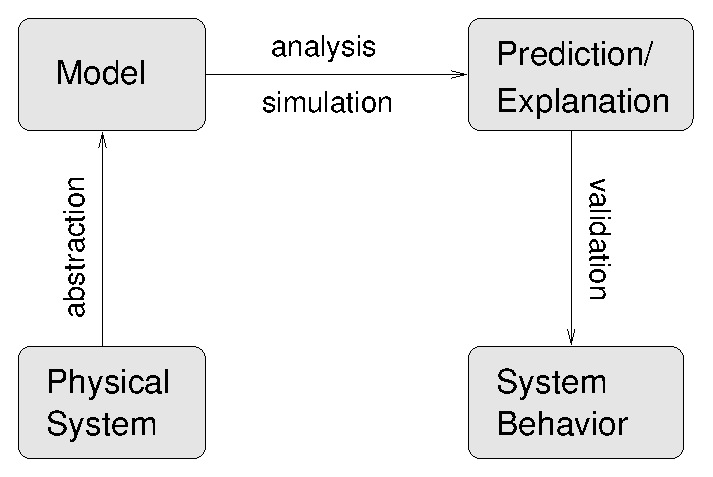
\includegraphics[height=1.5in]{figs/model.eps}}

A {\bf model} is a simplified description of a physical system. The
process of building a model is called {\bf abstraction}. In this
context, ``abstract'' is the opposite of ``realistic;'' an abstract
model bears little direct resemblance to the physical system it
models, in the same way that abstract art does not directly depict
objects in the real world. A realistic model is one that includes
more details and corresponds more directly to the real world.

Abstraction involves making justified decisions about which factors to
include in the model and which factors can be simplified or ignored.
For example, in the duck problem, we took into account the density of
the duck and the buoyancy of water, but we ignored the buoyancy of the
duck due to displacement of air and the dynamic effect of paddling
feet. We also simplified the geometry of the duck by assuming that
the underwater parts of a duck are similar to a segment of a sphere.
And we used coarse estimates of the size and weight of the duck.

Some of these decisions are justifiable. The density of the duck
is much higher than the density of air, so the effect of buoyancy
in air is probably small. Other decisions, like the spherical
geometry, are harder to justify, but very helpful. The actual
geometry of a duck is complicated; the sphere model makes it possible
to generate an approximate answer without making detailed measurements
of real ducks.

A more realistic model is not necessarily better. Models are useful
because they can be analyzed mathematically and simulated
computationally. Models that are too realistic might be difficult to
simulate and impossible to analyze.

A model is successful if it is good enough for its purpose. If we
only need a rough idea of the fraction of a duck that lies below
the surface, the sphere model is good enough. If we need a more
precise answer (for some reason) we might need a more realistic
model.

% Einstein's actual quote: ``It can scarcely be denied that the supreme
% goal of all theory is to make the irreducible basic elements as simple
% and as few as possible without having to surrender the adequate
% representation of a single datum of experience.

%   * "On the Method of Theoretical Physics" The Herbert Spencer
%    Lecture, delivered at Oxford (10 June 1933); also published in
%    Philosophy of Science, Vol. 1, No. 2 (April 1934),
%    pp. 163-169. [thanks to Dr. Techie @ www.wordorigins.org and
%    JSTOR]

Checking whether a model is good enough is called {\bf validation}.
The strongest form of validation is to make a measurement of an
actual physical system and compare it to the prediction of a
model.

If that is infeasible, there are weaker forms of validation. One is
to compare multiple models of the same system. If they are
inconsistent, that is an indication that (at least) one of them is
wrong, and the size of the discrepancy is a hint about the reliability
of their predictions.

We have only seen one physical model so far, so parts of this
discussion may not be clear yet. We will come back to these topics
later, but first we should learn more about vectors.



\section{Vectors as input variables}

Since many of the built-in functions take vectors as arguments,
it should come as no surprise that you can write functions that
take vectors. Here's a simple (silly) example:

\begin{verbatim}
function res = display_vector(X)
  X
end
\end{verbatim}

There's nothing special about this function at all. The only
difference from the scalar functions we've seen is that I used
a capital letter to remind me that {\tt X} is a vector.

This is another example of a function that doesn't actually have
a return value; it just displays the value of the input variable:

\begin{verbatim}
octave:1> display_vector(1:3)
X = 1   2   3
\end{verbatim}

Here's a more interesting example that encapsulates the code
from Section~\ref{reduce} that adds up the elements of a vector:

\begin{verbatim}
function res = mysum(X)
  total = 0;
  for i=1:length(X)
    total = total + X(i);
  end
  res = total;
end
\end{verbatim}

I called it {\tt mysum} to avoid a collision with the built-in
function {\tt sum}, which does pretty much the same thing.

Here's how you call it from the Command Window:

\begin{verbatim}
octave:2> total = mysum(1:3)
total = 6
\end{verbatim}

Because this function has a return value, I made a
point of assigning it to a variable.


\section{Vectors as output variables}

There's also nothing wrong with assigning a vector to an output
variable. Here's an example that encapsulates the code from
Section~\ref{apply}:

\begin{verbatim}
function res = myapply(X)
  for i=1:length(X)
    Y(i) = X(i)^2
  end
  res = Y
end
\end{verbatim}

Ideally I would have changed the name of the output variable to
{\tt Res}, as a reminder that it is supposed to get a vector value,
but I didn't.

Here's how {\tt myapply} works:

\begin{verbatim}
octave:1> V = myapply(1:3)
V = 1   4   9
\end{verbatim}

\begin{ex}
Write a function named {\tt find\_target} that
encapsulates the code, from Section~\ref{search}, that finds the
location of a target value in a vector.
\end{ex}


\section{Vectorizing your functions}

Functions that work on vectors will almost always work on scalars
as well, because Octave considers a scalar to be a vector with
length 1.

\begin{verbatim}
octave:1> mysum(17)
ans = 17

octave:2> myapply(9)
ans = 81
\end{verbatim}

Unfortunately, the converse is not always true. If you write
a function with scalar inputs in mind, it might not work on vectors.

But it might! If the operators and functions
you use in the body of your function work on vectors, then your
function will probably work on vectors.

For example, here is the very first function we wrote:

\begin{verbatim}
function res = myfunc (x)
  s = sin(x)
  c = cos(x)
  res = abs(s) + abs(c)
end
\end{verbatim}

And lo! It turns out to work on vectors:

\begin{verbatim}
octave:3> Y = myfunc(1:3)
Y = 1.3818  1.3254  1.1311
\end{verbatim}

At this point, I want to take a minute to acknowledge that I
have been a little harsh in my presentation of Octave, because
there are a number of features that I think make life harder
than it needs to be for beginners. But here, finally,
we are seeing features that show Octave's strengths.

Some of the other functions we wrote don't work on vectors,
but they can be patched up with just a little effort. For example,
here's {\tt hypotenuse} from Section~\ref{hypotenuse}:

\begin{verbatim}
function res = hypotenuse(a, b)
  res = sqrt(a^2 + b^2);
end
\end{verbatim}

This doesn't work on vectors because the \verb+^+ operator
tries to do matrix exponentiation, which only works on
square matrices.

\begin{verbatim}
octave:1> hypotenuse(1:3, 1:3)
??? Error using ==> mpower
Matrix must be square.
\end{verbatim}

But if you replace \verb+^+ with the elementwise operator
\verb+.^+, it works!

\begin{verbatim}
octave:1> A = [3,5,8];
octave:1> B = [4,12,15];
octave:1> C = hypotenuse(A, B)

C = 5  13  17
\end{verbatim}
 
In this case, it matches up corresponding elements from the two
input vectors, so the elements of {\tt C} are the hypotenuses of
the pairs $(3,4)$, $(5,12)$ and $(8,15)$, respectively.

In general, if you write a function using only elementwise
operators and functions that work on vectors, then the new
function will also work on vectors.


\section{Sums and differences}

Another common vector operation is {\bf cumulative sum}, which takes a
vector as an input and computes a new vector that contains all of the
partial sums of the original. In math notation, if $V$ is the
original vector, then the elements of the cumulative sum, $C$, are:

\[ C_i = \sum_{j=1}^i V_j \]

In other words, the $i$th element of $C$ is the sum of the first
$i$ elements from $V$. Octave provides a function named {\tt cumsum}
that computes cumulative sums:

\begin{verbatim}
octave:1> V = 1:5
V = 1   2   3   4   5

octave:2> C = cumsum(V)
C = 1   3   6  10  15
\end{verbatim}

\begin{ex}
Write a function named {\tt cumulative\_sum} that uses
a loop to compute the cumulative sum of the input vector.
\end{ex}

The inverse operation of {\tt cumsum} is {\tt diff}, which computes
the difference between successive elements of the input vector.

\begin{verbatim}
octave:3> D = diff(C)
D = 2   3   4   5
\end{verbatim}

Notice that the output vector is shorter by one than the input
vector. As a result, Octave's version of {\tt diff} is not
exactly the inverse of {\tt cumsum}. If it were, then we would
expect {\tt cumsum(diff(X))} to be {\tt X}:

\begin{verbatim}
octave:4> cumsum(diff(V))
ans = 1   2   3   4
\end{verbatim}

But it isn't.

\begin{ex}
Write a function named {\tt mydiff} that computes the
inverse of {\tt cumsum}, so that {\tt cumsum(mydiff(X))} and
{\tt mydiff(cumsum(X))} both
return {\tt X}.
\end{ex}


\section{Products and ratios}

The multiplicative version of {\tt cumsum} is {\tt cumprod},
which computes the {\bf cumulative product}. In math notation,
that's:

\[ P_i = \prod_{j=1}^i V_j \]

In Octave, that looks like:

\begin{verbatim}
octave:1> V = 1:5
V = 1   2   3   4   5

octave:2> P = cumprod(V)
P = 1   2   6  24  120
\end{verbatim}

\begin{ex}
Write a function named {\tt cumulative\_prod} that uses
a loop to compute the cumulative product of the input vector.
\end{ex}

Octave doesn't provide the multiplicative version
of {\tt diff}, which would be called {\tt ratio}, and which would
compute the ratio of successive elements of the input vector.

\begin{ex}
Write a function named {\tt myratio} that computes the
inverse of {\tt cumprod}, so that {\tt cumprod(myratio(X))} and
{\tt myratio(cumprod(X))} both
return {\tt X}.

You can use a loop, or if you want to be clever, you can take
advantage of the fact that $e^{\ln a + \ln b} = a b$.

If you apply {\tt myratio} to a vector that contains Fibonacci
numbers, you can confirm that the ratio of successive elements
converges on the golden ratio, $(1+\sqrt{5})/2$ (see
Exercise~\ref{fibratio}).
\end{ex}



\section{Existential quantification}

It is often useful to check the elements of a vector to see if there
are any that satisfy a condition. For example, you might want to
know if there are any positive elements. In logic, this condition
is called {\bf existential quantification}, and it is denoted with
the symbol $\exists$, which is pronounced ``there exists.'' For example,
this expression

\[ \exists x \mbox{~in~} S: x>0 \]

means, ``there exists some element $x$ in the set $S$ such that
$x>0$.'' In Octave it is natural to express this idea with a logical
function, like {\tt exists}, that returns 1 if there is such an
element and 0 if there is not.

\begin{verbatim}
function res = exists(X)
  for i=1:length(X)
    if X(i) > 0
      res = 1;
      return
    end
  end
  res = 0;
end
\end{verbatim}

We haven't seen the {\tt return} statement before; it is similar
to {\tt break} except that it breaks out of the whole function, not
just the loop. That behavior is what we want here because as soon
as we find a positive element, we know the answer (it exists!) and
we can end the function immediately without looking at the rest
of the elements.

If we exit at the end of the loop, that means we didn't find what
we were looking for (because if we had, we would have hit the
{\tt return} statement).



\section{Universal quantification}

Another common operation on vectors is to check whether {\em all}
of the elements satisfy a condition, which is known to
logicians as {\bf universal quantification} and denoted with
the symbol $\forall$ which is pronounced ``for all.'' So this
expression

\[ \forall x \mbox{~in~} S: x>0 \]

means ``for all elements, $x$, in the set $S$, $x>0$.''

A slightly silly way to evaluate this expression in Octave is to
count the number of elements that satisfy the condition.
A better way is to reduce the problem to
existential quantification; that is, to rewrite

\[ \forall x \mbox{~in~} S: x>0 \]

as

\[ \sim \exists x \mbox{~in~} S: x \le 0 \]

Where $\sim \exists$ means ``does not exist.''
In other words, checking that all the elements are positive is
the same as checking that there are no elements 
that are non-positive.

\begin{ex}
Write a function named {\tt forall} that
takes a vector and returns 1 if all of the elements are positive
and 0 if there are any non-positive elements.
\end{ex}




\section{Logical vectors}

When you apply a logical operator to a vector, the result is a {\bf
logical vector}; that is, a vector whose elements are the logical
values 1 and 0.

\begin{verbatim}
octave:1> V = -3:3
V = -3  -2  -1   0   1   2   3

octave:2> L = V>0
L = 0   0   0   0   1   1   1
\end{verbatim}

In this example, {\tt L} is a logical vector whose elements
correspond to the elements of {\tt V}. For each positive element of
{\tt V}, the corresponding element of {\tt L} is 1.

Logical vectors can be used like flags to store the state of
a condition. They are also often used with the {\tt find} function,
which takes a logical vector and returns a vector that contains
the indices of the elements that are ``true.''

Applying {\tt find} to {\tt L} yields

\begin{verbatim}
octave:3> find(L)
ans = 5   6   7
\end{verbatim}

which indicates that elements 5, 6 and 7 have the value 1.

If there are no ``true'' elements, the result is an empty vector.

\begin{verbatim}
octave:4> find(V>10)
ans = [](1x0)
\end{verbatim}

This example computes the logical vector and passes it as an
argument to {\tt find} without assigning it to an intermediate
variable. You can read this version abstractly as ``find
the indices of elements of {\tt V} that are greater than 10.''

We can also use {\tt find} to write {\tt exists} more concisely:

\begin{verbatim}
function res = exists(X)
  L = find(X>0)
  res = length(L) > 0
end
\end{verbatim}

\begin{ex}
Write a version of {\tt forall} using {\tt find}.
\end{ex}


\section{Glossary}

\begin{description}

\item[top-level function:] The first function in an M-file;
it is the only function that can be called from the Command
Window or from another file.

\item[helper function:] A function in an M-file that is not
the top-level function; it only be called from another function
in the same file.

\item[physical modeling:] A process
for making predictions about physical systems and explaining their
behavior.

\item[physical system:] Something in the real world that we are
interested in studying.

\item[model :] A simplified description of a
physical system that lends itself to analysis or simulation.

\item[abstraction:] The process of building a model by making
decisions about what factors to simplify or ignore.

\item[validation:] Checking whether a model is adequate for its
purpose.

\item[existential quantification:] A logical condition that expresses
the idea that ``there exists'' an element of a set with a certain
property.

\item[universal quantification:] A logical condition that expresses
the idea that all elements of a set have a certain property.

\item[logical vector:] A vector, usually the result of applying a logical
operator to a vector, that contains logical values 1 and 0. 


\end{description}

%\section{Exercises}

%\begin{ex}
%\end{ex}

% 
% % chap08 - Ordinary differential equations
\include{chapters/ode}
% 
% % chap09 - Systems of ODEs
\include{chapters/syst_ode}
% 
% % chap10 - Second-order systems
% chap10 - Second-order systems
% Last edited:

\chapter{Second-order systems}


\section{Nested functions}

In the Section~\ref{funfiles}, we saw an example of an M-file with
more than one function:

\begin{verbatim}
function res = duck()
  error = error_func(10)
end

function res = error_func(h)
  rho = 0.3;   % density in g / cm^3
  r = 10;     % radius in cm
  res = ...
end
\end{verbatim}

Because the first function ends before the second begins, they are at
the same level of indentation. Functions like these are {\bf
parallel}, as opposed to {\bf nested}. A nested function is
defined inside another, like this:

\begin{verbatim}
function res = duck()
  error = error_func(10)

  function res = error_func(h)
    rho = 0.3;   % density in g / cm^3
    r = 10;     % radius in cm
    res = ...
  end
end
\end{verbatim}

The top-level function, {\tt duck}, is
the {\bf outer function} and {\tt error\_func} is
an {\bf inner function}.

Nesting functions is useful because the variables of the outer
function can be accessed from the inner function. This is not
possible with parallel functions.

In this example, using a nested function makes it possible to
move the parameters {\tt rho} and {\tt r} out of {\tt error\_func}.

\begin{verbatim}
function res = duck(rho)
  r = 10;
  error = error_func(10)

  function res = error_func(h)
    res = ...
  end
end
\end{verbatim}

Both {\tt rho} and {\tt r} can be accessed from {\tt error\_func}.
By making {\tt rho} an input argument, we made it easier to test
{\tt duck} with different parameter values.



\section{Newtonian motion}

Newton's second law of motion is often written like this

\[ F = ma \]

where $F$ is the net force acting on a object, $m$ is the mass
of the object, and $a$ is the resulting acceleration of the object.
In a simple case where the object is moving along a straight line,
$F$ and $a$ are scalars, but in general they are vectors.

Even more generally, if $F$ and $a$ vary in time, then they can
be thought of as functions that return vectors; that is, $F$ is
a function and the result of evaluating $F(t)$ is a vector that
describes the net force at time $t$. So a more explicit way to
write Newton's law is

\[ \forall t: \vec{F}(t) = m \vec{a}(t) \]

The arrangement of this equation suggests that if you know $m$ and $a$
you can compute force, which is true, but in most physical
simulations it is the other way around. Based on a physical
model, you know $F$ and $m$, and compute $a$.

So if you know acceleration, $a$, as a function of time, how do you
find the position of the object, $p$? Well, we know that acceleration
is the second derivative of position, so we can write a differential
equation

\[ p_{tt} = a \]

Where $a$ and $p$ are functions of time that return vectors,
and $p_{tt}$ is the second time derivative of $p$.

Because this equation includes a second derivative, it is a second-order
ODE. {\tt ode45} can't solve this equation in this form, but by
introducing a new variable, $v$, for velocity, we can rewrite it as
a system of first-order ODEs.

\begin{eqnarray*}
p_t &=& v \\
v_t &=& a
\end{eqnarray*}

The first equation says that the first derivative of $p$ is $v$; the
second says that the derivative of $v$ is $a$.


\section{Freefall}
\label{freefall}

Let's start with a simple example, an object in freefall in a vacuum
(where there's no air resistance). Near the surface of the earth, the
acceleration of gravity is $g = -9.8$ $m/s^2$, where the minus sign
indicates that gravity pulls down.

If the object falls straight down (in the same direction as gravity),
we can describe its position with a scalar value, altitude. So
this will be a one-dimensional problem, at least for now.

Here is a rate function we can use with {\tt ode45} to solve
this problem:

\begin{verbatim}
function res = freefall(t, X)
  p = X(1);   % the first element is position
  v = X(2);   % the second element is velocity

  dpdt = v;             
  dvdt = acceleration(t, p, v);

  res = [dpdt; dvdt];  % pack the results in a column vector
end

function res = acceleration(t, p, v)
  g = -9.8;   % acceleration of gravity in m/s^2
  res = g;
end
\end{verbatim}

The first function is the rate function. It gets {\tt t} and
{\tt X} as input variables, where the elements of {\tt X} are understood
to be position and velocity. The return value from {\tt freefall}
is a (column) vector that contains the derivatives of position
and velocity, which are velocity and acceleration, respectively. 

Computing $p_t$ is easy because we are given velocity
as an element of {\tt X}. The only thing we have to compute is
acceleration, which is what the second function does.

{\tt acceleration} computes acceleration as a function of time,
position and velocity. In this example, the net acceleration is
a constant, so we don't really have to include all this information
yet, but we will soon.

Here's how to run {\tt ode45} with this rate function:

\begin{verbatim}
octave:1> ode45(@freefall, [0, 30], [4000, 0])
\end{verbatim}
 
As always, the first argument is the function handle, the second
is the time interval (30 seconds) and the third is the initial
condition: in this case, the initial altitude is 4000 meters and
the initial velocity is 0. So you can think of the ``object'' a
a skydiver jumping out of an airplane at about 12,000 feet.

Here's what the result looks like:

\beforefig \centerline{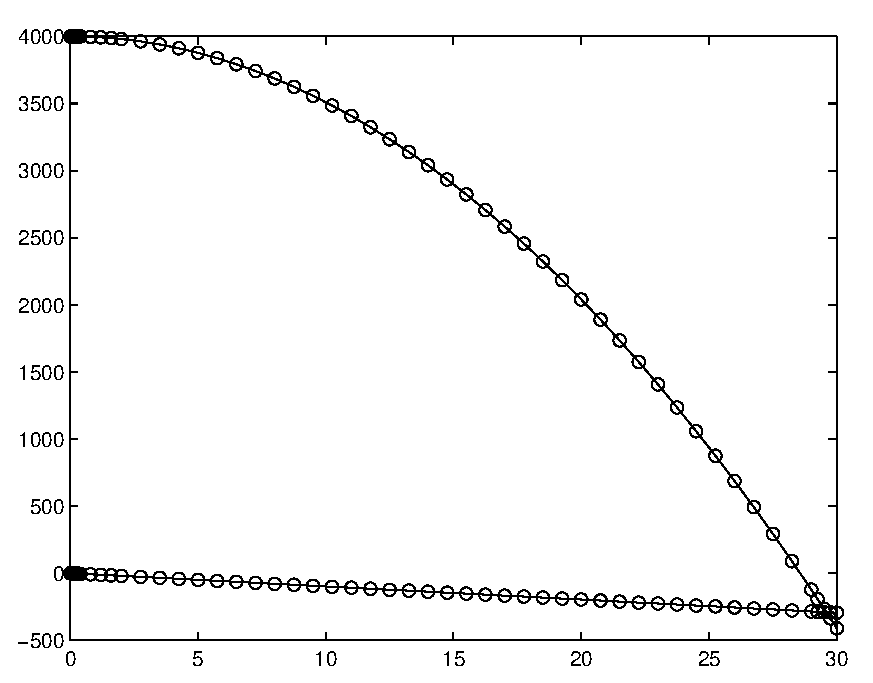
\includegraphics[height=2in]{figs/freefall.eps}}

The bottom line shows velocity starting at zero and dropping
linearly. The top line shows position starting at 4000 m and
dropping parabolically (but remember that this parabola
is a function of time, not a ballistic trajectory).

Notice that {\tt ode45} doesn't know where the ground is, so the
skydiver keeps going through zero into negative altitude. We will
address this issue later.


\section{Air resistance}

To make this simulation more realistic, we can add air resistance.
For large objects moving quickly through air, the force due to air
resistance, called ``drag,'' is proportional to $v^2$:

\[ F_{drag} = c v^2 \]

Where $c$ is a drag constant that depends on the density of
air, the cross-sectional area of the object and
the surface properties of the object. For purposes of this
problem, let's say that $c = 0.2$.

To convert from force to acceleration, we have to know mass, so let's
say that the skydiver (with equipment) weighs 75 kg.

Here's a version of {\tt acceleration} that takes air resistance
into account (you don't have to make any changes in {\tt freefall}:

\begin{verbatim}
function res = acceleration(t, p, v)
  a_grav = -9.8;       % acceleration of gravity in m/s^2
  c = 0.2;          % drag constant
  m = 75;           % mass in kg
  f_drag = c * v^2;      % drag force in N
  a_drag = f_drag / m;    % drag acceleration in m/s^2
  res = a_grav + a_drag;   % total acceleration
end
\end{verbatim}

The sign of the drag force (and acceleration) is positive as
long as the object is falling, the direction of the drag force is
up.
The net
acceleration is the sum of gravity and drag. Be careful when you
are working with forces and accelerations; make sure you only add
forces to forces or accelerations to accelerations. In my code,
I use comments to remind myself what units the values are in.
That helps me avoid nonsense like adding forces to accelerations.

Here's what the result looks like with air resistance:

\beforefig \centerline{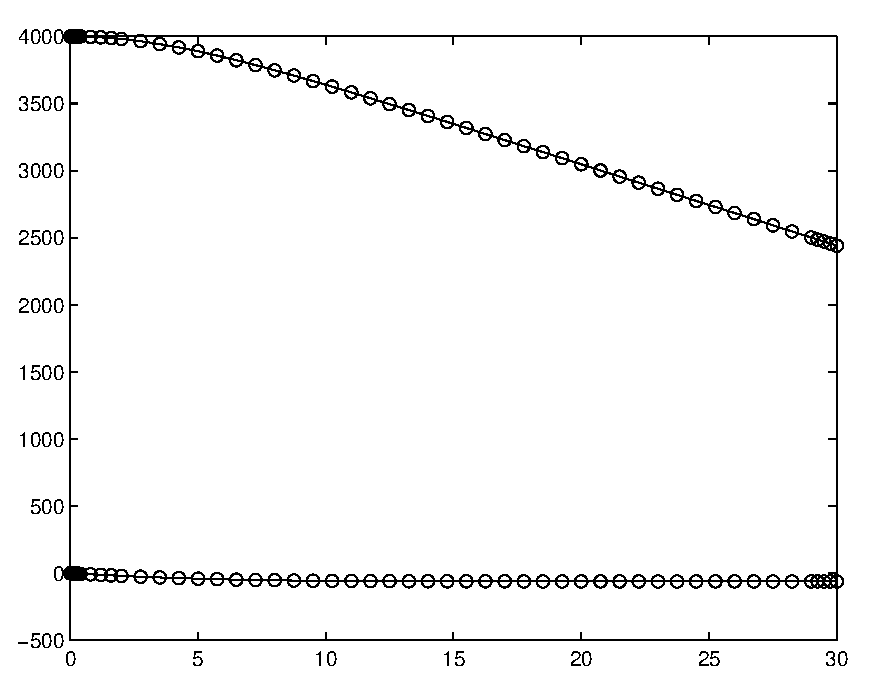
\includegraphics[height=2in]{figs/freefall2.eps}}

Big difference! With air resistance, velocity increases until
the drag acceleration equals $g$; after that, velocity is a constant,
known as ``terminal velocity,'' and position decreases linearly
(and much more slowly than it would in a vacuum). To examine
the results more closely, we can assign them to variables


\begin{verbatim}
octave:1> [T, M] = ode45(@freefall, [0, 30], [4000, 0]);
\end{verbatim}

And then read the terminal position and velocity:

\begin{verbatim}
octave:1> M(end,1)

ans = 2.4412e+03     % altitude in meters

octave:1> M(end,2)

ans = -60.6143      % velocity in m/s
\end{verbatim}

\begin{ex}
Increase the mass of the skydiver, and confirm that
terminal velocity increases. This relationship is the source of the
intuition that heavy objects fall faster; in air, they do!
\end{ex}


\section{Parachute!}

In the previous section, we saw that the terminal velocity of a $75
kg$ skydiver is about 60 $m/s$, which is about 130 mph. If you hit
the ground at that speed, you would almost certainly be killed.
That's where parachutes come in.

\begin{ex}
Modify {\tt acceleration} so that after 30 seconds of
free-fall the skydiver deploys a parachute, which (almost) instantly
increases the drag constant to 2.7.

What is the terminal velocity now? How long (after deployment) does
it take to reach the ground?
\end{ex}


\section{Two dimensions}
\label{projectile}

So far we have used {\tt ode45} for a system of first-order
equations and for a single second-order equation. The next logical
step is a system of second-order equations, and the next logical example
is a projectile. A ``projectile'' is an object propelled
through space, usually toward, 
and often to the detriment of,
a target.

If a projectile stays in a plane, we can think of the system as
two-dimensional, with $x$ representing the horizontal distance
traveled and $y$ representing the height or altitude. So now
instead of a skydiver, think of a circus performer being fired
out of a cannon.

According to the
Wikipedia\footnote{\url{http://en.wikipedia.org/wiki/Human_cannonball}},
the record distance for a human cannonball is 56.5 meters (almost 186
feet).

Here is a general framework for computing the trajectory of a projectile
in two dimensions using {\tt ode45}:

\begin{verbatim}
function res = projectile(t, W)
  P = W(1:2);
  V = W(3:4);

  dPdt = V;             
  dVdt = acceleration(t, P, V);

  res = [dPdt; dVdt];
end

function res = acceleration(t, P, V)
  g = -9.8;       % acceleration of gravity in m/s^2
  res = [0; g];
end
\end{verbatim}

The second argument of the rate function is a vector, {\tt W}, with
four elements. The first two are assigned to {\tt P}, which
represents position; the last two are assigned to {\tt V}, which
represents velocity.
{\tt P} and {\tt V} are vectors with
elements for the $x$ and $y$ components.

The result from
{\tt acceleration} is also a vector; ignoring air resistance
(for now), the acceleration in the $x$ direction is 0; in
the $y$ direction it's $g$.
Other than that, this code is similar to what we saw in
Section~\ref{freefall}.

If we launch the human projectile from an initial height of
3 meters, with velocities 40 m/s and 30 m/s in the $x$ and $y$
directions, the {\tt ode45} call looks like
this:

\begin{verbatim}
ode45(@projectile, [0,10], [0, 3, 40, 30]);
\end{verbatim}

And the result looks like this:

\beforefig \centerline{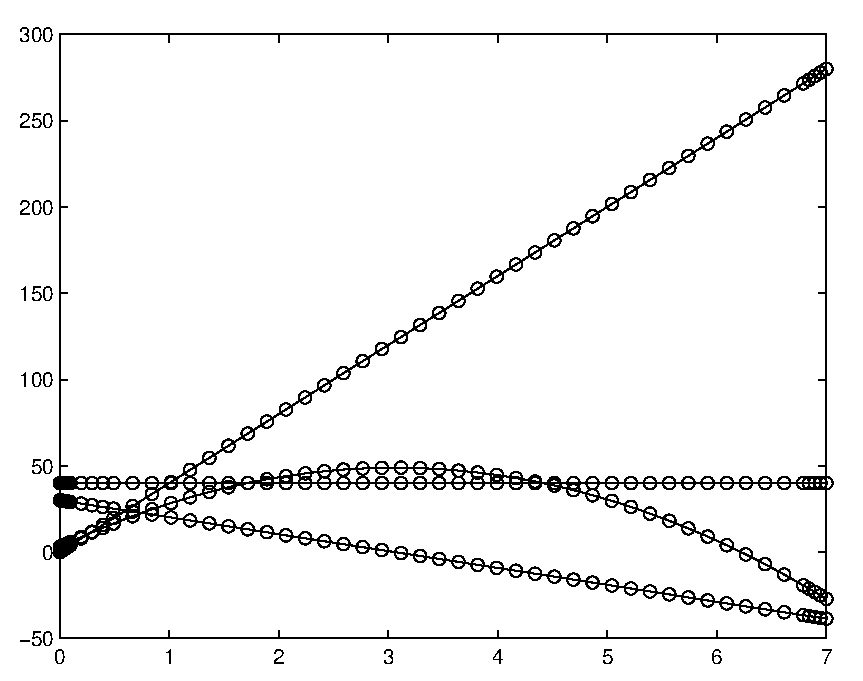
\includegraphics[height=2in]{figs/proj1.eps}}

You might have to think a little to figure out which line is
which. It looks like the flight time is about 6 seconds.

\begin{ex}
Extract the $x$ and $y$ components of
position, plot the trajectory of the projectile, and estimate the
distance traveled.
\end{ex}

\begin{ex}
Add air resistance to this simulation. In
the skydiver scenario, we estimated that the drag constant was
$0.2$, but that was based on the assumption that the skydiver is
falling flat. A human cannonball, flying head-first, probably
has a drag constant closer to $0.1$. What initial velocity
is needed to achieve the record flight distance of 65.6 meters?
Hint: what is the optimal launch angle?
\end{ex}


\section{What could go wrong?}

What could go wrong? Well, {\tt vertcat} for one. To explain
what that means, I'll start with {\bf catenation}, which is
the operation of joining two matrices into a larger matrix.
``Vertical catenation'' joins the matrices by stacking them on
top of each other; ``horizontal catenation'' lays them
side by side.

Here's an example of horizontal catenation with row vectors:

\begin{verbatim}
octave:1> x = 1:3

x = 1   2   3

octave:1> y = 4:5

y = 4   5

octave:1> z = [x, y]

z = 1   2   3   4   5
\end{verbatim}

Inside brackets, the comma operator performs horizontal catenation.
The vertical catenation operator is the semi-colon. Here is an
example with matrices:

\begin{verbatim}
octave:1> X = zeros(2,3)

X = 0   0   0
   0   0   0

octave:1> Y = ones(2,3)

Y = 1   1   1
   1   1   1

octave:1> Z = [X; Y]

Z = 0   0   0
   0   0   0
   1   1   1
   1   1   1
\end{verbatim}

These operations only work if the matrices are the same size along
the dimension where they are glued together. If not, you get:

\begin{verbatim}
octave:1> a = 1:3

a = 1   2   3

octave:1> b = a'

b = 1
   2
   3

octave:1> c = [a, b]
??? Error using ==> horzcat
All matrices on a row in the bracketed expression must have the 
 same number of rows.

octave:1> c = [a; b]
??? Error using ==> vertcat
All rows in the bracketed expression must have the same 
number of columns.
\end{verbatim}

In this example, {\tt a} is a row vector and {\tt b} is a column
vector, so they can't be catenated in either direction.

Reading the error messages, you probably guessed that {\tt horzcat}
is the function that performs horizontal catenation, and likewise
with {\tt vertcat} and vertical catenation.

These operations are relevant to {\tt projectile} because of the
last line, which packs {\tt dPdt} and {\tt dVdt} into the
output variable:

\begin{verbatim}
function res = projectile(t, W)
  P = W(1:2);
  V = W(3:4);

  dPdt = V;             
  dVdt = acceleration(t, P, V);

  res = [dPdt; dVdt];
end
\end{verbatim}

As long as both {\tt dPdt} and {\tt dVdt} are column vectors,
the semi-colon performs vertical catenation, and the result is
a column vector with four elements. But if either of them is a
row vector, that's trouble.

{\tt ode45} expects the result from {\tt projectile} to be a
column vector, so if you are working with {\tt ode45}, it is
probably a good idea to make {\em everything} a column vector.

In general, if you run into problems with {\tt horzcat} and {\tt
vertcat}, use {\tt size} to display the dimensions of the operands,
and make sure you are clear on which way your vectors go.


\section{Glossary}

\begin{description}

\item[parallel functions:] Two or more functions defined side-by-side,
so that one ends before the next begins.

\item[nested function:] A function defined inside another function.

\item[outer function:] A function that contains another function
definition.

\item[inner function:] A function defined inside another function
definition. The inner function can access the variables of the
outer function.

\item[catenation:] The operation of joining two matrices end-to-end to
form a new matrix.


\end{description}

\section{Exercises}

\begin{ex}
\label{baseball}

The flight of a baseball is governed by three forces: gravity,
drag due to air resistance, and Magnus force due to spin. If
we ignore wind and Magnus force, the path of the baseball stays
in a plane, so we can model it as a projectile in two
dimensions.

A simple model of the drag of a baseball is:
%
\[ F_d = -\frac{1}{2} ~ \rho ~ v^2 ~ A ~ C_d ~ \hat{V}  \]
%
where $F_d$ is a vector that represents the force on the baseball due
to drag, $C_d$ is the drag coefficient (0.3 is a reasonable choice),
$\rho$ is the density of air (1.3 kg/m$^3$ at sea level), $A$ is the
cross sectional area of the baseball (0.0042 m$^2$), $v$ is the
magnitude of the velocity vector, and $\hat{V}$ is a unit vector in
the direction of the velocity vector. The mass of the baseball is
$0.145$ kg.

For more information about drag, see
\url{http://en.wikipedia.org/wiki/Drag_(physics)}.

\begin{itemize}

\item Write a function that takes the initial velocity of the baseball
and the launch angle as input variables, uses {\tt ode45} to compute
the trajectory, and returns the range (horizontal distance in flight)
as an output variable.

\item Write a function that takes the initial velocity of the baseball
as an input variable, computes the launch angle that maximizes
the range, and returns the optimal angle and range as output variables.
How does the optimal angle vary with initial velocity?

\item When the Red Sox won the World Series in 2007, they played the
Colorado Rockies at their home field in Denver, Colorado. Find an
estimate of the density of air in the Mile High City. What effect
does this have on drag? Make a prediction about what effect this will
have on the optimal launch angle, and then use your simulation to test
your prediction.

\item The Green Monster in Fenway Park is about 12 m high and about 97
m from home plate along the left field line. What is the minimum
speed a ball must leave the bat in order to clear the monster
(assuming it goes off at the optimal angle)? Do you think it is
possible for a person to stand on home plate and throw a
ball over the Green Monster?

\item The actual drag on a baseball is more complicated than what is
captured by our simple model. In particular, the drag coefficient
varies with velocity. You can get some of the details from {\em The
Physics of Baseball}\footnote{Robert K. Adair, Harper Paperbacks, 3rd
Edition, 2002.}; you also might find information on the web.
Either way, specify a more realistic model of drag and modify your
program to implement it. How big is the effect on your computed
ranges? How big is the effect on the optimal angles?

\end{itemize}

\end{ex}


% 
% % chap11 - Optimization and interpolation
\include{chapters/opt_and_interp}
% 
% % chap12 - Vectors as vectors
\include{chapters/vect_as_vect}


\end{document}